%!TEX root = ../../../super_main.tex

\chapter{Collaboration}
\todo{NIKLAS + DONEHOLMIUM: Skriv motivation for de to samarbejder med grupperne og kort hvad det gik ud på. Skriv også at der har været en del samarbejde generelt men en masse små ting. Vi har udvalgt de opgaver hvor der var mest pair programming involveret.}

The following collaboration sections are the shared work of ours and another group. We sat down together and resolved shared, or similar, issues across the projects. During the development of \giraf, this is far from the only collaboration with other groups, however, the documented cases are the only collaborations that have been well documented. While collaborating with other groups, we used methods like pair programming and code reviews. This chapter will describe the collaborations that we have done with the other groups.

\todo{NIKLAS + DONEHOLMIUM: END}

%!TEX root = ../../../super_main.tex
\section{Collaboration with Group SW606F15}
\label{sec:collaboration_with_group_sw606f15}

After a general GUI design meeting, a new sequence deletion method was suggested by the customers. Sequences are used in some of the applications that are being developed by the other GUI groups. Sequences are lists of pictograms that should be viewed in chronological order, when then represent a behavior/action sequence which the citizen can execute. This could for example be the order in which a citizen should dress, e.g. putting on his socks before shoes. \todo{Add a visual example of a sequence}. 
\\\\
The application \emph{Sequence} contains a set of different sequences. It is required of the application that different sequences may be removed. Previously when deleting sequences, the user would have to click a button to enter a ``Delete mode'' where, instead of clicking sequences to view them, clicks would delete the sequence. The customers requested the option to long-press a sequence to enter a ``Multi-selection mode'' where they were able to select multiple sequences in order to delete them. When a sequence is long pressed, the main menu is supposed to enter this mode and a trashcan button should appear in the top-bar. It should be possible to select and deselect sequences through regular press once inside the selection mode. It should furthermore be possible to deselect and exit the selection mode upon pressing the back button in the action bar.
\\\\
In our project, we had need for a feature just like this one, which instead of selecting sequences was focused around selecting pictograms inside categories. To quickly overcome this task, we grouped up with SW606f15, in order to resolve their issue first so we could implement the same structure in the two applications. The difference between the two projects is that our solution should only select a single item with a regular press, where theirs should be able to select multiple when initiated by a long-press.
\\\\
Previously, their project was based around the use of sequence objects and their respective ids to create views that represent the sequences. This resulted in not being able to find the view that belonged to the individual sequence, without passing both sequence and its view when using them in a method. This made it impossible to create the deselection feature when pressing the back button, since the back button was overriding the original \androidinline{onBackPressed} method, which does not take any parameters.
\\\\ 
Because of this we decided to implement a new data structure for their project which contains both a sequence and its respective view. This new structure made it possible to access the views that were selected and then deselect them when the back-button is pressed. 
\\\\
We furthermore implemented this using adapters as previously described, to improve performance when iterating through the list of sequences. This method of implementation could be directly transferred into our own project with minimal changes.

%!TEX root = ../../../super_main.tex

\section{Collaboration with Group SW613F15}
\label{sec:collaboration_with_group_sw613f15}

After the recent handover of \gc from group \emph{SW604F15} (us) to \emph{SW613F15}, it was discovered that a component in \ps (developed by \emph{SW613F15}) was not consistent with the design implemented in the \launcher (implemented by \emph{SW604F15}) regarding showing of multiple items, applications and pictograms respectively. This inconsistency can be seen in \figref{fig:collab_with_group_13}.

\begin{figure}[!htbp]
    \centering

    \begin{subfigure}[t]{0.75\textwidth}
        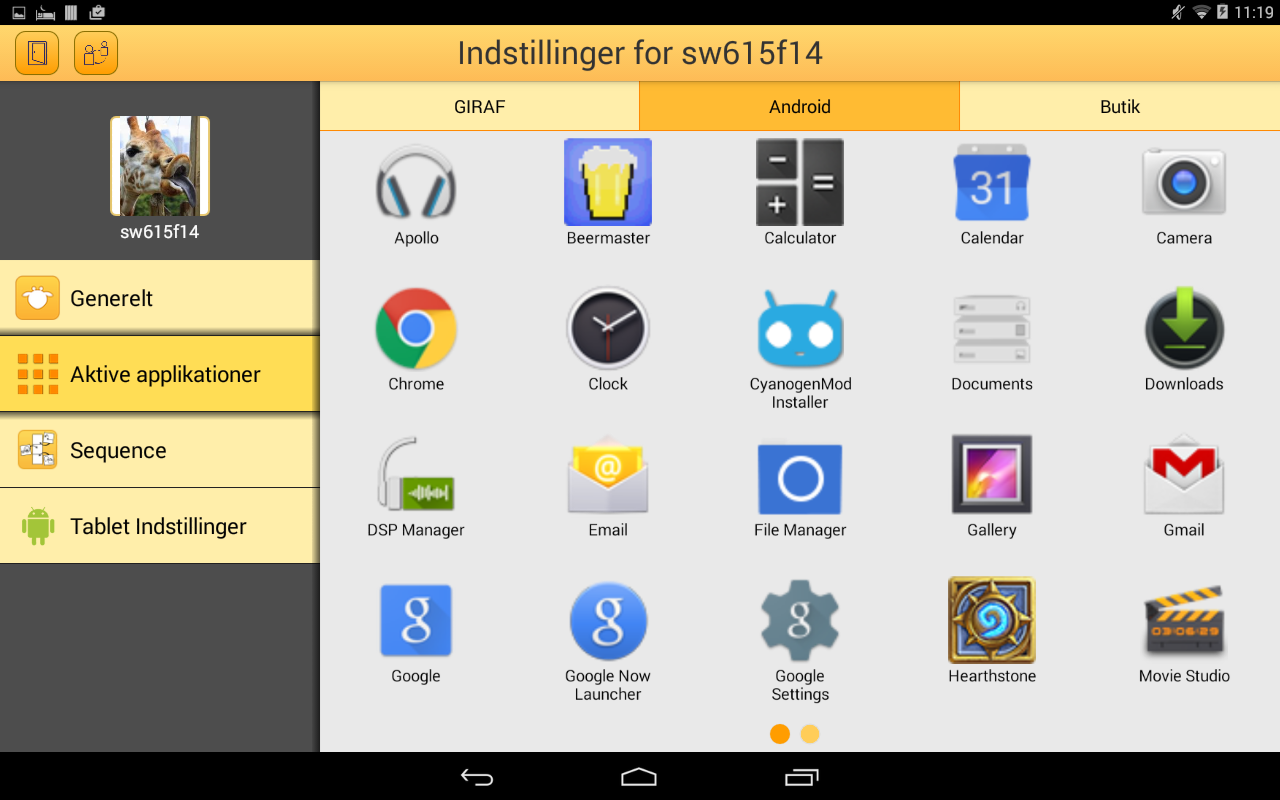
\includegraphics[width=\textwidth]{sprint_three/collab_with_group_13/launcher.png}
        \caption{The \launcher application}
        \label{fig:collab_with_group_13_launhcer}
        \vspace*{1cm}
    \end{subfigure}
    \hfill
    \begin{subfigure}[t]{0.75\textwidth}
        \includegraphics[width=\textwidth]{sprint_three/collab_with_group_13/pictosearch.png}
        \caption{The old \ps application}
        \label{fig:collab_with_group_13_pictosearch}
    \end{subfigure}
    
    \caption{Problem visualized}
    \label{fig:collab_with_group_13}
\end{figure}

Since \emph{SW604F15} had already spent some time on implementing a viewpager for this purpose, a solution for \ps was made in collaboration by these groups. A slight implementation difference was that the viewpager in the launcher is implementing using a \androidinline{FragmentAdapter}, whereas the viewpager in \ps is implemented using \androidinline{GridView}s. This soloution was though found to be inconsistent in regards to the other displays of pictograms and it was decided that there should be distinction between how applications should be presented and how pictograms and profile pictures should be presented. For this reasons we assisted \emph{SW613F15} to implemented a \androidinline{GridView} like the one implemented in \ct. The final result of \ps can be seen in \figref{fig:pictosearch}.


\begin{figure}[!htbp]
    \centering
    \includegraphics[width=0.75\textwidth]{sprint_three/pictosearch}
    \caption{Resulting application look for \ps}
    \label{fig:pictosearch}
\end{figure}